\documentclass[a4paper,pdf]{article}
\usepackage{hyperref}
\usepackage{pdfpages} % http://mirror.unl.edu/ctan/macros/latex/contrib/pdfpages/pdfpages.pdf
\usepackage{booktabs} 



\usepackage[utf8]{inputenc}
\usepackage{amsmath}
\usepackage{graphicx}
\usepackage[colorinlistoftodos]{todonotes} % handig voor commentaar: gebruik \todo{}, zie ftp://ftp.fu-berlin.de/tex/CTAN/macros/latex/contrib/todonotes/todonotes.pdf
\usepackage{listings}
\usepackage{pdfpages}
\usepackage{tcolorbox}
\usepackage{float}
\usepackage{caption}
\usepackage{subcaption}


% when writing in Dutch
\usepackage[dutch]{babel}
\selectlanguage{dutch}

% Voor de references
\usepackage[round,authoryear]{natbib}
\usepackage{cite}
\usepackage[normalem]{ulem}
\usepackage{hyperref}
\usepackage[normalem]{ulem}
\useunder{\uline}{\ul}{}
\usepackage{amsmath}
\usepackage{bm}
\usepackage{url}

\usepackage{tikz}

\begin{document}




%%% DIT IS DE TITLE PAGE VOOR INFORMATIEKUNDE NIET VOOR AI OF INFORMATICA! 
%% GEBRUIK VOOR AI OF INFORMATICA JE EIGEN TITLEPAGE TEMPLATES\


\begin{center}

\vspace{2.5cm}

% [CHANGE] The title of your thesis. If your thesis has a subtitle, then this
% should appear right below the main title, in a smaller font.
\begin{Huge}
Title of the thesis
\end{Huge}

\vspace{1.5cm}

% [CHANGE] Your full name. In case of multiple names, you can include their
% initials as well, e.g. "Jan G.J. van der Wegge".
Sebastiaan T. Verhaar\\
% [CHANGE] Your student ID, as this has been assigned to you by the UvA
% administration.
10177914

\vspace{1.5cm}

% [DO NOT CHANGE]
Bachelor thesis\\
% [CHANGE] Whether your Bachelor thesis is 6 ECTS (regular) or 9 ECTS (Honours
% programme).
Credits: 12 EC

\vspace{0.5cm}

% [DO NOT CHANGE] The name of the educational programme.
Bachelor Opleiding Informatiekunde

\vspace{0.25cm}

% [DO NOT CHANGE] The addess of the educational programme.
University of Amsterdam\\
Faculty of Science\\
Science Park 904\\
1098 XH Amsterdam

\vspace{4cm}

\emph{Supervisor}\\
% [CHANGE] The name of your supervisor. Include the titles of your supervisor,
% as well as the initials for *all* of his/her first names.
Dr. M. J. Marx

\vspace{0.25cm}

% [CHANGE] The address of the institute at which your supervisor is working.
% Be sure to include (1) institute (is appropriate), (2) faculty (if
% appropriate), (3) organisation name, (4) organisation address (2 lines).
ILPS, IvI\\
Faculty of Science\\
University of Amsterdam\\
Science Park 904\\
1098 XH  Amsterdam

\vspace{1.5cm}

% [CHANGE] The date at which you will finalize and submit your thesis.
2016-06-26

\end{center}



\pagebreak

\tableofcontents

\pagebreak

\begin{abstract}
% [CHANGE] 
\end{abstract}


\pagebreak


% Here you input all your sections in seperate files

\section{Introduction}
\label{sec:intro}

Wikipedia is een voorbeeld van de grootste online community van collaborerende mensen op het internet. Op Wikipedia zijn er veel users die edits maken op pagina's. Zij maken nieuwe pagina's, bewerken pagina's of controleren bewerkingen van andere users. Achter elke pagina schuilt ook een discussiepagina. Deze discussiepagina's dienen voor coordinatie, discussies en communicaties tussen \textit{Wikipedians}. In tegenstelling tot andere veel andere websites, zijn discussiepagina's op Wikipedia dus niet bedoelt voor entertainment, maar om tot een consensus te komen wat zal zorgen tot verbetering van Wikipedia pagina's \citep{laniado2011wikipedians}.  Echter, uit een vragenlijst bleek dat minder dan 20\% van deze Wikipedians vrouw is \citep{glott2010analysis}. Dit grote verschil tussen aantal mannen en aantal vrouwen binnen deze Wikipedians heeft veel aandacht gekregen van zowel de media als andere onderzoekers. Gender onderzoeksliteratuur \citep{collier2012conflict} suggereert dat dit verschil kan komen door:
\begin{enumerate}
    \item Het hoge aantal conflicten in discussies
    \item Afkeer van kritische omgevingen
    \item Te kort aan zelfvertrouwen bij het aanpassen van andermans werk.
\end{enumerate}  
Er zijn al een aantal onderzoeken gedaan naar het analyseren van de inhoud van Wikipedia discussiepagina's \citep{viegas2007talk} en de structuur van de discussiepagina's van Wikipedia \citep{laniado2011wikipedians}, maar nog niet naar het verschil tussen mannenlijke en vrouwlijke verschillen op discussiepagina's van Wikipedia. In deze thesis wordt er gekeken naar het verschil in gebruik van de discussiepagina's van Wikipedia tussen mannelijke en vrouwlijke Wikipedians.



\subsection{Onderzoeksvragen}
Om verschil tussen mannen en vrouwen op Wikipedia talkpages beter te bekijken, zijn er een aantal onderzoeksvagen opgesteld. 

\begin{description}
\item[Onderzoeksvraag 1] Zijn er vaak discussies tussen mannelijke gebruikers en vrouwelijke gebruikers op discussiepagina's?

\item[Onderzoeksvraag 2] Is het taalgebruik van mannelijke gebruikers negatiever dan het taalgebruik van vrouwelijke gebruikers op discussiepagina's van Wikipedia?

\subsection{Inhoud van thesis}


\begin{comment}
\begin{itemize}
\item Bevat je onderzoeksvraag (of vragen)
\item Plaatst je vraag in de bestaande literatuur.
\end{itemize}

Je onderzoeksvraag is leidend voor je hele scriptie. Alles wat je doet moet uiteindelijk terug te voeren zijn op 1 doel: het beantwoorden van die vraag. 

Typisch zal je het dan ook zo doen:

Mijn onderzoeksvraag is onderverdeeld in de volgende deelvragen:

\begin{description}
\item[RQ1] \ldots We   beantwoorden deze vraag  door het volgende te doen/ antwoord op de volgende vragen te vinden/ \ldots
\begin{enumerate}
\item Vragen op dit niveau kan je echt beantwoorden, en dat doe je in je Evaluatie sectie~\ref{sec:eva}.
\end{enumerate}
\item[RQ2] \ldots
\item[RQ3] \ldots
\end{description}

Je Evaluatie sectie~\ref{sec:eva} bevat evenveel subsecties als je deelvragen hebt. En in elke sectie beantwoord je dan die deelvraag met behulp van de vragen op het onderste niveau.

In je conclusies kan je dan je hoofdvraag gaan beantwoorden op basis van al het eerder vergaarde bewijs.


\paragraph{Overview of thesis}
Hier geef je even kort weer wat in elke sectie staat.

\end{comment}


\section{Related Work}
\label{sec:rel}

Er is al eerder onderzoek gedaan naar het verschil in gender op Wikipedia. Door middel van vragenlijsten is onderzocht naar het verschil in aantal mannelijke en vrouwelijke Wikipedia editors. Hieruit kwam dat ongeveer 16,1\% van de editors op de online encyclopedie van het vrouwelijke geslacht is \citep{hill2013wikipedia}. Binnen Amerika lag dit wel een beetje hoger, namelijk 22,7\% van de editors was hier van het vrouwelijke geslacht. Hoewel Wikipedia meer artikelen heeft over vrouwen dan andere online encyclopedia zoals Britannica, is het zo dat binnen Wikipedia zelf relatief weinig artikelen gaan over vrouwen ten opzichten van artikelen over mannen \citep{reagle2011gender}. Hieruit lijkt het redelijk duidelijk dat vrouwen worden ondervertegenwoordigd. Het is daarom belangrijk om af te vragen waardoor dit komt. Ligt het bijvoorbeeld aan persoonlijke voorkeur, aantrekkelijkheid of discriminatie. Door deze oorzaak te begrijpen kan worden ingegrepen om balans te herstellen. 

\subsection{Kritiek}
Hoewel Wikipedia bekent staat dat alle mensen iets kunnen 'bijdragen' aan de gemeenschap, is het vaak zo dat 'bijdragen' staat voor het verwijderen of aanpassen van andermans werk. 'Samenwerken' betekent dus niet altijd dat iedereen collectief nieuwe informatie produceert. Vaak is 'samenwerken' het feit dat mensen het werk van onbekende anderen lezen, corrigeren en soms ook verwijderen. Er is al eerder onderzocht dat als kinderen, jongens sneller kiezen voor competitieve spelletjes, terwijl meisjes sneller kiezen voor spelletjes zonder een winnaar \citep{campbell2013mind}. Een reden hiervan is dat mannen meer houden van competitie. Vrouwen reageren ook anders op kritiek dan mannen. Mannen reageren minder op positieve of negatieve feedback dan vrouwen \citep{roberts1994gender}. Vrouwen krijgen meer zelfvertrouwen van positieve feedback terwijl mannen relatief onaangetast blijven. Bij het ontvangen van negatieve kritiek wordt het zelfvertrouwen van vrouwen aanzienlijk verlaagd terwijl dit van mannen wederom onaangetast blijft \citep{roberts1994gender}. Vrouwen gaven ook aan 31\% banger te zijn voor negatieve houdingen ten opzichten van hun werk op Wikipedia \citep{collier2012conflict}. Een reden voor het lage aantal vrouwelijke editors op Wikipedia zou dus kunnen zijn dat mannen negatiever zijn dan vrouwen. 
\begin{description}
\item[Onderzoeksvraag 1] Is het taalgebruik van mannelijke gebruikers negatiever dan het taalgebruik van vrouwelijke gebruikers op discussiepagina's van Wikipedia?
\end{description}

\subsection{Conflict}
Behalve de kritieke sfeer tussen Wikipedia editors, is er ook een hoog niveau aan conflicten. Hoewel het lijkt dat er veel wordt samengewerkt op Wikipedia, staan de discussiepagina's vol met \textit{edit-warring}: een fenomeen waar editors proberen andere edits op te heffen \citep{cassell2011editwars}. Volgens Cassell moeten editors erop aandringen dan hun standpunt de enige geldige is. Eerder onderzoek heeft al aangetoond dat vrouwen sneller geneigd zijn om conflicten te vermijden dan man \citep{brewer2002gender}. Ook ervaren vrouwen sneller angst en verhoogde hartslag bij conflicterende situaties \citep{smith1998agency}. Eerder onderzoek toonde ook aan dat vrouwen onderhandelingen en conflict zelfs vermijden als het gaat om hoge kosten. Een vrouw is bereid ongeveer \$1300,- meer te betalen voor een auto om onderhandelingen te vermijden \citep{babcock2009women}. Omdat Wikipedia's discussiepagina's grotendeels zijn gebaseerd op het oplossen van conflicten, persoonlijke discussies en onderhandelingen om tot een consensus te komen, zouden de verschillen in gender om mee te doen aan deze activiteiten de impact van contributie kunnen be\"{i}nvloeden.
\begin{description}
\item[Onderzoeksvraag 2] Zijn er vaak discussies tussen mannelijke gebruikers en vrouwelijke gebruikers op discussiepagina's?
\end{description}

\section{Methodology}
\label{sec:meth}


\subsection{Description of the data}
Data verzameling en beschrijving van de data

Hoe is de data verzameld, en hoe heb jij die data verkregen?


Wat staat er in de data? Niet alleen maar een technisch verhaal, maar ook inhoudelijk. DE lezer moet een goed idee krijgen over de technische inhoud en wat het betekent.

\pagebreak
\subsection{Wat plotjes en tabelletjes}

Zie het IPython Notebook \url{PandasAndLatex.ipynb} voor de code om vanuit pandas een poltje op te slaan en een dataframe als tabel op te slaan. Het werkt ideaal! 

De interrupties van Wilders staan beschreven in Figure~\ref{fig:wilders} en Tabel~~\ref{tab:Wilders}.


\begin{figure}
\begin{center}
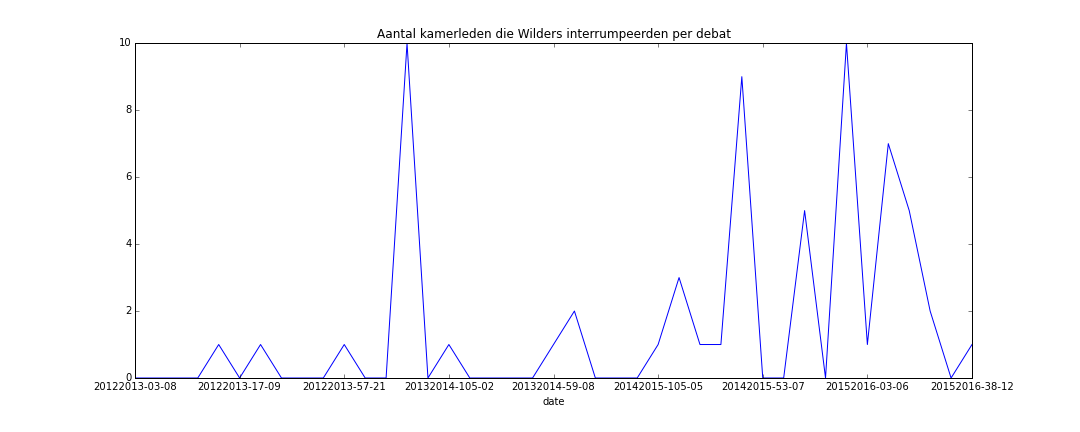
\includegraphics[width=\linewidth]{WildersPlot.png}
\caption{\label{fig:wilders} Aantal interrupties van Wilders in de Tweede Kamer door de tijd (periode 2012-2016).}
\end{center}
\end{figure}


\pagebreak

\begin{table}[h]
\begin{footnotesize}
\begin{tabular}{lrl}
\toprule
{} &  indegree &                               interruptie\_volgorde \\
date            &           &                                                    \\
\midrule
20122013-03-08  &         0 &                                                    \\
20122013-07-16  &         0 &                                                    \\
20122013-100-03 &         0 &                                                    \\
20122013-100-06 &         0 &                                                    \\
20122013-17-06  &         1 &                         Pechtold-Pechtold-Pechtold \\
20122013-17-09  &         0 &                                                    \\
20122013-21-04  &         1 &                         Pechtold-Pechtold-Pechtold \\
20122013-22-08  &         0 &                                                    \\
20122013-32-06  &         0 &                                                    \\
20122013-48-23  &         0 &                                                    \\
20122013-57-21  &         1 &  Pechtold-Pechtold-Pechtold-Pechtold-Pechtold-P... \\
20122013-76-03  &         0 &                                                    \\
20122013-76-06  &         0 &                                                    \\
20132014-05-02  &        10 &  Roemer-Roemer-Van Haersma Buma-Van Haersma Bum... \\
20132014-06-04  &         0 &                                                    \\
20132014-105-02 &         1 &  Pechtold-Pechtold-Pechtold-Pechtold-Pechtold-P... \\
20132014-105-06 &         0 &                                                    \\
20132014-14-03  &         0 &                                                    \\
20132014-14-06  &         0 &                                                    \\
20132014-52-18  &         0 &                                                    \\
20132014-59-08  &         1 &                               Klaver-Klaver-Klaver \\
20142015-02-08  &         2 &  Pechtold-Pechtold-Pechtold-Pechtold-Pechtold-P... \\
20142015-03-06  &         0 &                                                    \\
20142015-09-09  &         0 &                                                    \\
20142015-100-05 &         0 &                                                    \\
20142015-105-05 &         1 &                                  Pechtold-Pechtold \\
20142015-111-04 &         3 &  Pechtold-Pechtold-Pechtold-Pechtold-Pechtold-P... \\
20142015-111-07 &         1 &                                  Pechtold-Pechtold \\
20142015-39-71  &         1 &                                  Pechtold-Pechtold \\
20142015-41-07  &         9 &  Samsom-Samsom-Pechtold-Pechtold-Pechtold-Kuzu-... \\
20142015-53-07  &         0 &                                                    \\
20142015-61-23  &         0 &                                                    \\
20142015-79-07  &         5 &  Klaver-Klaver-Klaver-Gesthuizen-Gesthuizen-Ges... \\
20142015-95-06  &         0 &                                                    \\
20152016-02-07  &        10 &  Pechtold-Pechtold-Pechtold-Pechtold-Slob-Slob-... \\
20152016-03-06  &         1 &       Pechtold-Pechtold-Pechtold-Pechtold-Pechtold \\
20152016-14-02  &         7 &  Klaver-Klaver-Roemer-Roemer-Roemer-Roemer-Sams... \\
20152016-14-05  &         5 &  Van Haersma Buma-Van Haersma Buma-Van Haersma ... \\
20152016-27-03  &         2 &  Segers-Segers-Segers-Segers-Kuzu-Kuzu-Kuzu-Kuz... \\
20152016-38-10  &         0 &                                                    \\
20152016-38-12  &         1 &                                        Klein-Klein \\
\bottomrule
\end{tabular}

\end{footnotesize}
\caption{\label{tab:Wilders} Door wie werd Wilders onderbroken en hoe vaak per debat.}
\end{table}


\pagebreak
\subsection{Methods}
Hoe je je vraag gaat beantwoorden.


Dit is de langste sectie van je scriptie. 

Als iets erg technisch wordt kan je een deel naar de Appendix verplaatsen. 

Probeer er een lopend verhaal van te maken.

Het is heel handig dit ook weer op te delen nav je deelvragen:

\subsubsection{RQ1}

\subsubsection{RQ2}
\section{Evaluation}
\label{sec:eva}

Met een subsectie voor elke deelvraag.

In hoeverre is je vraag beantwoord?

Een mooie graphic/visualisatie is hier heel gewenst.

Hou het kort maar krachtig.
\section{Conclusions}
\label{sec:conc}

Hierin beantwoord je jouw hoofdvraag op basis van het eerder vergaarde bewijs.



\subsection{Acknowledgements}
Hier kan je bedanken wie je maar wilt.

% your refs

%\bibliographystyle{plain}
%\bibliography{MyThesis}

\appendix

%\input{appendix}


\section{Slides}

% Example
%
\includepdf[nup=2x3 , pages=-]{sargent-lecture_slides.pdf}

%Include alle literatuur
\bibliography{literature.bib}{}
\bibliographystyle{plainnat}
 
\end{document}
